\documentclass{beamer}

\useinnertheme{metropolis}
\useoutertheme{metropolis}
\usecolortheme{metropolis}
\usefonttheme{professionalfonts}         % Use metropolis theme

\usepackage{fontspec}
\setsansfont{Fira Sans Light}
\setmonofont{Fira Mono}
\setmainfont{Fira Sans Light}

\usepackage[bibstyle=unified, citestyle=unified, backend=biber]{biblatex}
\addbibresource{fdsl.bib}

\usepackage{longtable}
\usepackage{tipa}
\usepackage{booktabs}
\usepackage{tikz}
\usepackage{tikz-qtree}
\usepackage{expex}
\usepackage[normalem]{ulem}
\usepackage{xcolor}
\usepackage{float}
\usepackage{etoolbox}
\usepackage{multirow}
\usepackage{graphicx}
\usepackage{wrapfig}
\usepackage{subfig}
\usepackage{mathabx}
\usepackage{hyperref}


	\usetikzlibrary{matrix}
	\usetikzlibrary{positioning}
	\usetikzlibrary{tikzmark}
	\usetikzlibrary{decorations.shapes}
	\usetikzlibrary{arrows}
	\usetikzlibrary{decorations.pathreplacing,backgrounds}

	\hypersetup{
		colorlinks=true,
		linkcolor=black,
		citecolor=magenta,
		filecolor=black,
    		urlcolor=black,
	}

\tikzset{mytree/.style={baseline=(top.base),
level distance=2.5em, sibling distance=4em, align=center,
parent anchor=south, child anchor=south, anchor=north}}

\lingset{numoffset=1ex, belowglpreambleskip=0ex, aboveglftskip=0ex, belowexskip=2ex, aboveexskip=2ex} % gloss formatting


\renewcommand*{\bibfont}{\small}
\setbeamertemplate{bibliography item}{}


\AtBeginSection[]{
  \begin{frame}
  \vfill
  \centering
  \usebeamerfont{title}\insertsectionhead\par%
  \vfill
  \end{frame}
}


\title{Stress shift in Slavic and Phase Theory}
\date{5/10/2022 \\ }
\author{Alexandra Shikunova, Daniar Kasenov}

\begin{document}

\maketitle

	\section{Introduction}

	\begin{frame}{Intro}
	
		\begin{itemize}
			\item This talk reviews and sketches a phonological analysis of structural conditions on stress shift in Russian PPs 

			\item Slides and general info can be found at github.com/antidanyar

			\item {\small The results of the project "Languages of Russia: morphosyntax and its interaction with other modules”, carried out within the framework of the Basic Research Program at the National Research University Higher School of Economics (HSE University) in 2022, are presented in this work.}

		\end{itemize}

	\end{frame}

	\begin{frame}{Prosody of Russian prepositions}

		Russian prepositions are clitics, the host bears the stress (\ref{ex:basic1}). However, the stress shifts to the preposition sometimes (\ref{ex:basic2}).
		
		\begin{minipage}{.48\textwidth}
		\pex\label{ex:basic1}
				\a po pólyu\\
				`through a/the field'
				\a na rúku’\\
				`on one's arm'
		\xe
		\end{minipage}
		\hfill
		\begin{minipage}{.49\textwidth}
		\pex\label{ex:basic2}
				\a pó polyu\\
				`through a/*the field'
				\a ná ruku\\
				`on one's arm'
		\xe
		\end{minipage}

	\end{frame}
	
	\begin{frame}{Lexical restrictions}
	
	The stress shift is lexically restricted wrt. both nouns and prepositions (\cite{Gribanova:2013}).
	
	\begin{minipage}{.49\textwidth}
		\pex\label{ex:basic1}
				\a pó polyu\\
				`through a/*the field'
				\a *nád polem\\
				(`above a field')
		\xe
		\end{minipage}
		\hfill
		\begin{minipage}{.5\textwidth}
		\pex\label{ex:basic2}
				\a *pó polyane\\
				(`through a meadow')
				\a *ná ladon’\\
				(`on one's arm')
		\xe
		\end{minipage}
		
	We aim to explain the distribution of shifted/non-shifted stress in those PPs that allow for both variants.
	
	\end{frame}

	\begin{frame}{Goals of the talk}

		\begin{itemize}
			\item Review the properties of the stress shift
			\item Review the solution to it by \textcite{Gribanova:2013}
			\item Suggest an analysis that assumes a transparent syntax-phonology interface based on spell-out (\cite{Scheer:2012}; \cite{Scheer:2016})
		\end{itemize}

	\end{frame}

	\section{Structural conditions on the stress shift}

	\begin{frame}{"Locality" of the shift}
	
	Russian stress shift in general, it appears, is only possible from the nearest syllable -- the first syllable of the noun/verb/numeral.
	
	\begin{itemize}
			\item \emph{ne bylá} / *\emph{né byla} `she was not' 
			\item \emph{ne býlo} / \emph{né bylo} `it was not' 
			\item \emph{ne býl} / \emph{né byl} `he was not' 
	\end{itemize}
	
	This is true of the stress shift in PPs as well.
	
		\ex
				po doróge/ *pó doroge\\
				`down a road'
		\xe
	
	\end{frame}

	\begin{frame}{Non-branching requirement}

		The noun that undergoes stress shift cannot host any modifiers, even in a postnominal position.
		
		\begin{itemize}
			\item no adjectives
			\item no possessors
			\item no participle or relative clauses
		\end{itemize}

	\end{frame}

	\begin{frame}
	
		\ex
			\begingl 
				\glpreamble Adjective//
				\gla *ya gulayu pó polyu raznotsvetnomu//
				\glb I walk through field multi-colored//
				\glft `I walk through a multi-colored field.'//
			\endgl
		\xe

	\end{frame}
	
	\begin{frame}
	
		\ex
			\begingl 
				\glpreamble Possessor (inanimate)//
				\gla *pó polyu bitvy//
				\glb through field battle.GEN//
				\glft `through a battlefield'//
			\endgl
		\xe
		
		\ex
			\begingl 
				\glpreamble Possessor (animate)//
				\gla *ná ruku Natashi//
				\glb on arm Natasha.GEN//
				\glft `onto Natasha's arm'//
			\endgl
		\xe


	\end{frame}

	\begin{frame}
	
		\ex
			\begingl 
				\glpreamble Participle clause//
				\gla *ya gulayu pó polyu, ukrashennomu tsvetami//
				\glb I walk through field decorated by.flowers//
				\glft `I walk through a field decorated by flowers.'//
			\endgl
		\xe
		
		\ex
			\begingl 
				\glpreamble Relative clause//
				\gla ya gulayu pó lesu, chto sazhal moy ded//
				\glb I walk through forest which planted my grandpa//
				\glft `I walk through the forest, which my grandpa planted.'//
			\endgl
		\xe

	\end{frame}
	
	\begin{frame}{Argument-adjunct asymmetry}

		\textcite{Blumenfeld:2011}: Prepositions whose spatial or temporal semantics is transparent are
more likely to undergo stress shift than those which are idiosyncratically selected by the verb; likely has to do with the argument-adjunct distinction.

	\end{frame}

	\begin{frame}
		
		\pex PP with the stress shift should be adjoined
			\a \begingl
			\gla vystupat' zá gorod//
			\glb {step out} outside city//
			\glft `To step out of the city'//
			\endgl

			\a \begingl
			\gla *vystupat' zá gorod//
			\glb {defend} outside city//
			\glft `To defend the city' \\(in the context of city as a concept, even)//
			\endgl
		\xe

	\end{frame}

	\begin{frame}{Summarizing properties}

		\begin{itemize}

			\item The nominal phrase should be sufficiently small

			\item The PP should be an adjunct

			\item Stress may shift only if the nominal is stress-initial

		\end{itemize}

	\end{frame}

	\section{Solution by Gribanova and Blumenfeld}

	\begin{frame}{The prosodic structure}

		\textcite{Gribanova:2013}: stress shift $\Leftarrow$ all syllables are contained in a single prosodic word

		\begin{tikzpicture}[mytree, inv/.style={overlay, coordinate}, sibling distance=4em, level distance=2em]
					\node(top) {$\omega$}
					child {node {$\sigma$}
						child {node {pó}}
					}
					child {node {$\sigma$}
							child {node {po}}
					}
					child {node {$\sigma$}
							child {node {lyu}}
					}
					;
	\end{tikzpicture}

	\end{frame}

	\begin{frame}{The prosodic structure}

		B\&G: no stress shift $\Leftarrow$ the preposition syllable is not contained in the same minimal prosodic word

		\begin{tikzpicture}[mytree, inv/.style={overlay, coordinate}, sibling distance=4em, level distance=2em]
					\node(top) {$\omega$}
					child {node {$\sigma$}
						child {node {po}}
					}
					child {node {$\omega$}
						child {node {$\sigma$}
							child {node {pó}}
						}
						child {node {$\sigma$}
							child {node {lyu}}
						}
					}
					;
	\end{tikzpicture}				

	\end{frame}

	\begin{frame}{Two prepositions}

		B\&G postulate two phonological spell-outs of the same preposition (in syntax); only one may clitisize in the minimal prosodic word

		\pex Insertion rules
				\a P $\leftrightarrow$ po- /\_\_ minimal N \hfill (cliticizes)
				\a P $\leftrightarrow$ po  \hfill (doesn't cliticize)
		\xe

	\end{frame}


	\begin{frame}{B\&G: major drawbacks}

		\begin{itemize}
		
			\item Two different phonological entities -- theoretically unfavorable
			
			\item The only property that's accounted for is the size of the nominal
	
			\item Given Bare Phrase Structure, how can the translation from syntax to phonology distinguish between minimal and maximal projections?

		\end{itemize}

	\end{frame}
	
%%%%%%%%%%%%%%%%%%%%%%%%%%%%%%%%%%%%%%%%%%%%%%%%%%%%%%%%%%%%%%%
%%%%%%%%%%%%%%%%%%%%%%%%%%%%%%%%%%%%%%%%%%%%%%%%%%%%%%%%%%%%%%%
%%%%%%%%%%%%%%%%%%%%%%%%%%%%%%%%%%%%%%%%%%%%%%%%%%%%%%%%%%%%%%%

	\section{Our analysis}

	\begin{frame}{Our assumptions}

		\begin{itemize}
			\item Morphosyntactic boundaries exist in phonology as a by-product of cyclic Spell-Out (\cite{Scheer:2016})

			\item Boundaries are encoded as empty CV units (\cite{Scheer:2012})

		\end{itemize}

	\end{frame}

	\begin{frame}{Tying together syntactic conditions}

		Recall: (a) nominal should be small; (b) PP should be an adjunct

		Our reformulation: the noun and the preposition should be in the same spell-out domain

	\end{frame}

	\begin{frame}{The spell-out condition}

		Smallness of the nominal: no phasal node inbetween P and N (like D)

		Adjunct requirement: if PP is an argument, the NP spells out before P due to the weak PIC

		If PP is an adjunct, it spells out together (\cite{Stepanov:2007}; \cite{Privoznov:2021})

		The syntactic result: stress shift results from the same-domainness of preposition and nominal, not via indirect formation of prosodic structure (as B\&G argue)

	\end{frame}

	\begin{frame}{The phonological side}
	
		One way or another, we need to tie together spell-out domains and stress assignment

		Procedural way: stress is assigned at the first spell-out (cf. \cite{Marvin:2013})

		Representational way: the spell-out domain boundary (empty CV) blocks stress assignment to the preposition

	\end{frame}

	\begin{frame}{Representational way}

		\textcite{Enguehard:2016}: Russian stress is represented by a CV unit on the \textbf{right} of the syllable

		\textcite{Enguehard:2014}: empty CV-as-boundary and empty CV-as-stress may be the same CV
		
 		That gives the prediction that preposition will always be stressed (not the case)

	\end{frame}

	\begin{frame}{Another stress system}

		\textcite{Faust:2018}: grid projection account based on two ideas

		(a) empty CVs may project

		(b) their grid markers are incorporated by contentful nuclei

		The problem: they assume that incorporation goes to the left (same wrong prediction)

	\end{frame}

	\begin{frame}{How to capture the word-initiality}

		We assume that words with word-initial stress have it due to stress assignment rules (Basic Accentuation Principle; \cite{Melvold:1989})

	Therefore, once the preposition is in the same domain (however we achieve that), it becomes the initial syllable

	\end{frame}

	\begin{frame}{Summary}

		Russian stress shift can be analysed only using the cyclic spellout without resorting to postulating distinct homophonous entites

		However, the precise phonological implementation is a compicated manner

	\end{frame}

	\begin{frame}

		Thank you!

		The slides and info can be found at github.com/antidanyar

	\end{frame}

	\begin{frame}[allowframebreaks]{References}
		\printbibliography[heading=none]
	\end{frame}


\end{document}